\documentclass[a4paper]{article}
% add (renew) commands

\usepackage[a4paper,top=1.3cm,bottom=2cm,left=1.5cm,right=1.5cm,marginparwidth=0.75cm]{geometry}

%\usepackage[margin=1.8cm]{geometry}         %!  фиксирует оступ на 2cm
\usepackage{xcolor}
\usepackage{hyperref} 
\definecolor{grey}{HTML}{666666}
\definecolor{linkcolor}{HTML}{0000CC}
\definecolor{urlcolor}{HTML}{006600}
\hypersetup{
    pdfstartview=FitH,  
    linkcolor=linkcolor,
    urlcolor=urlcolor, 
    colorlinks=true,
    citecolor=blue,
    unicode=true}
\usepackage[utf8]{inputenc}
\usepackage[russian]{babel}
\usepackage{graphicx}%для пикч
\usepackage{pgfplots}%для графиков
\pgfplotsset{compat=1.9}%тоже
\usepackage{amsfonts} %ШРИФТ ДЛЯ R
\usepackage{float} %размещение пикч
\usepackage{amsmath} %для aligned тип чтобы равно было посередине
\usepackage{wrapfig}
\usepackage{mathtext}
\usepackage{gensymb}
\usepackage{tabto}



\usepackage{listings}
\usepackage{color}

\definecolor{dkgreen}{rgb}{0,0.6,0}
\definecolor{gray}{rgb}{0.5,0.5,0.5}
\definecolor{mauve}{rgb}{0.58,0,0.82}

\lstset{frame=tb,
  language=c++,
  aboveskip=3mm,
  belowskip=3mm,
  showstringspaces=false,
  columns=flexible,
  basicstyle={\small\ttfamily},
  numbers=none,
  numberstyle=\tiny\color{gray},
  keywordstyle=\color{blue},
  commentstyle=\color{dkgreen},
  stringstyle=\color{mauve},
  breaklines=true,
  breakatwhitespace=true,
  tabsize=3
}
\begin{document}


\begin{center}
    \LARGE \textsc{Второе задание}
\end{center}

\hrule

\phantom{42}

\begin{flushright}
    \begin{tabular}{rr}
    % written by:
        \textbf{Автор}: 
        & Маллаев Руслае \\
        &\\
    % date:
        \textbf{От}: &
        \textit{\today}\\
    \end{tabular}
\end{flushright}

\thispagestyle{empty}
\tableofcontents





\section{RDF} % (fold)
\label{sec:rdf}


\begin{figure}[h]
\begin{center}
\begin{minipage}[h]{0.45\linewidth}
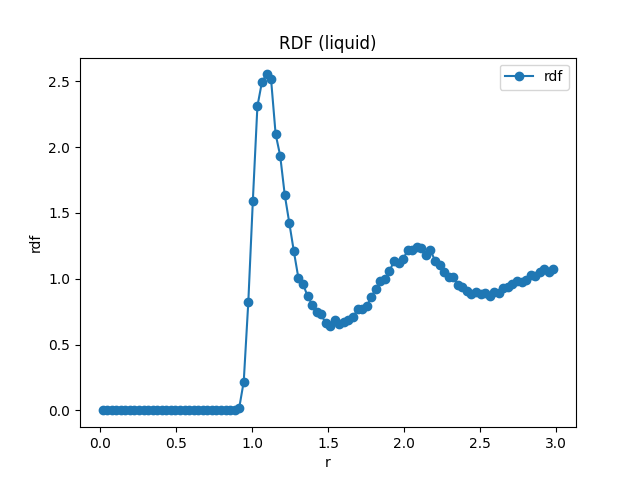
\includegraphics[width=1\linewidth]{rdfl.png}
\caption{RDF жидкости при $\rho=0.85$ и $T= 85 K$ } %% подпись к рисунку
\label{ris:experimoriginal} %% метка рисунка для ссылки на него
\end{minipage}
\hfill
\begin{minipage}[h]{0.45\linewidth}
\begin{center}
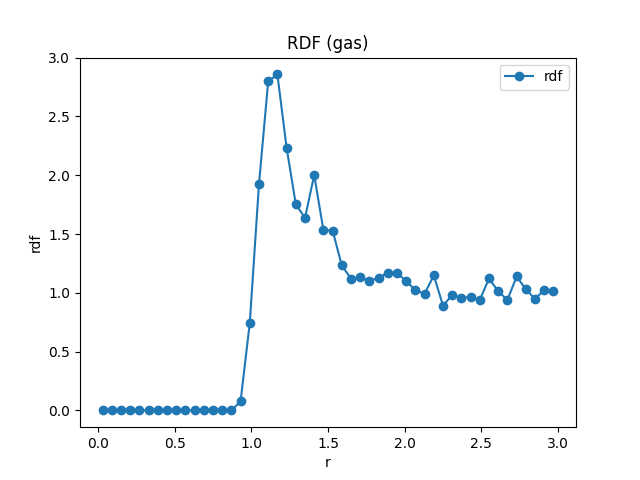
\includegraphics[width=1.1\textwidth]{rdf.png}
\caption{RDF газа при $\rho = 0.05$ и $T = 85 K$}
\end{center}
\end{minipage}
\end{center}
\end{figure}
Пики у нас получились у жидкости на 3,41 А, у газа на 3.83 А. У Yarnell на 3.76 А. Расхождение может быть обусловлено разными плотностями (сам он вроне не указал при каких).
% section rdf (end)
% section code (end)


\section{Автокореллятор} % (fold)
Усредняем по $m=30$ с промежутком $n=600$ шагов 
\label{sec:автокореллятор}
\begin{itemize}
\item жидкость $N=1000$ $dt=0.00005$ число шагов $Nt=100000$ $T=1.0$ $rho=0.85$   
\item газ $N=1000$ $dt=0.02$ число шагов $Nt=30000$ $T=1.2$ $rho=0.005$

\end{itemize}

\begin{figure}[h]
\begin{center}
\begin{minipage}[h]{0.45\linewidth}
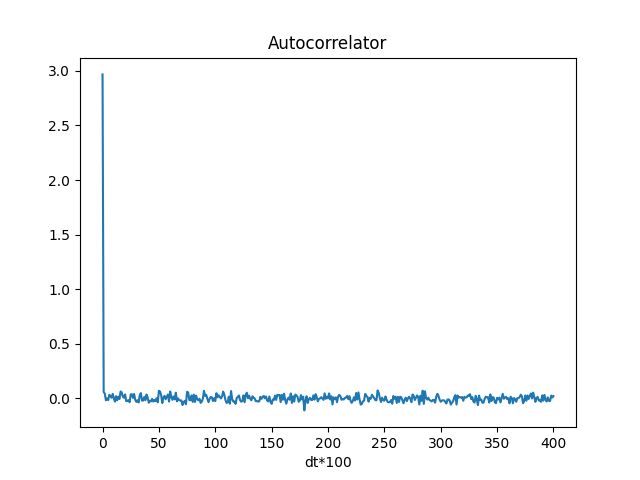
\includegraphics[width=1.1\linewidth]{vacfl.png}
\caption{Автокореллятор жидкости при $\rho=0.85$ и $T= 1.0$ } %% подпись к рисунку
\label{ris:experimoriginal} %% метка рисунка для ссылки на него
\end{minipage}
\hfill
\begin{minipage}[h]{0.45\linewidth}
\begin{center}
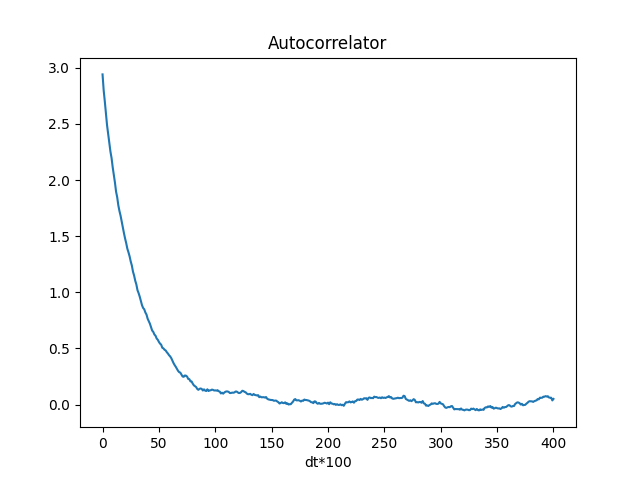
\includegraphics[width=1.1\textwidth]{vacf.png}
\caption{Автокореллятор газа при $\rho= 0.005$ и $T = 1.2$}
\end{center}
\end{minipage}
\end{center}
\end{figure}
Ну тут у нас в разреженном газе он не залезает в отрицательные значения, что ожидаемо. Для жидкости он очень резко падает, но последующие неровности скорее объясняются недостатком усреднения
% section автокореллятор (end)


\section{Диффузия методом Эйнштейна-Смолуховского} % (fold)
\label{sec:диффузия_методом_эйнштейна_смолуховского}
\subsection*{СКС}

\begin{figure}[H]
\begin{center}
\begin{minipage}[h]{0.45\linewidth}
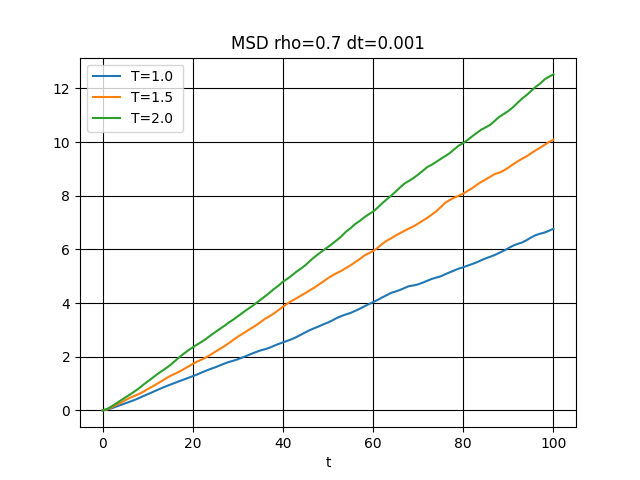
\includegraphics[width=1.1\linewidth]{msd.png}
\caption{СКС при $\rho=0.7$} %% подпись к рисунку
\label{ris:experimoriginal} %% метка рисунка для ссылки на него
\end{minipage}
\hfill
\begin{minipage}[h]{0.45\linewidth}
\begin{center}
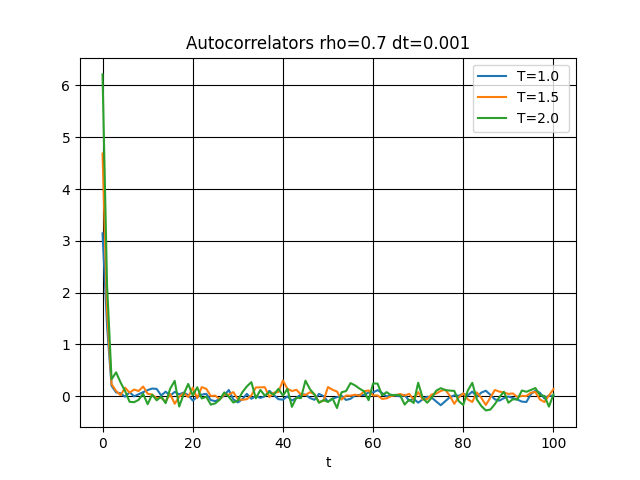
\includegraphics[width=1.1\textwidth]{vac.png}
\caption{Автокореллятор газа при $\rho= 0.7$}
\end{center}
\end{minipage}
\end{center}
\end{figure}


\subsection*{reference Rowley}
\begin{itemize}
    \item $\rho = 0.7$ $T = 1.0$ $D = 0.105$
    \item $\rho = 0.7$ $T = 1.5$ $D = 0.156$
    \item $\rho = 0.7$ $T = 2.1$ $D = 0.217$
\end{itemize}
На первом графике значения диффузии посчитаны по наклону, на втором представлены автокорреляторы. Как видим полученные значения по первому графику сходятся с погрешностью $\pm 10\%$. Теперь проинтегрируем их чтобы получить значения методом Эйнштейна-Смолуховского. Считал в LAMMPS, $dt = 0.005$ $N_{timesteps} = 20000$  усреднял по 30 фреймам. \\
Мои значения
\begin{itemize}
    \item $\rho = 0.7$ $T = 1.0$ $D = 0.117$
    \item $\rho = 0.7$ $T = 1.5$ $D = 0.167$
    \item $\rho = 0.7$ $T = 2.1$ $D = 0.215$
\end{itemize}
Ну тут тоже попали в значения с максимальной погрешностью $7\%$, так что все +- норм 




% section диффузия_методом_эйнштейна_смолуховского (end)

\section{Из первого задания} % (fold)
\label{sec:из_первого_задания}
Посчитаем диффузию по невязкам из первого задания. У одной модели было $dt = 0.001$ у другой $dt = 0.01$, диввузию считаем как $D = \frac{1}{12}\alpha$, где $\alpha$ наклон графика
\begin{center}
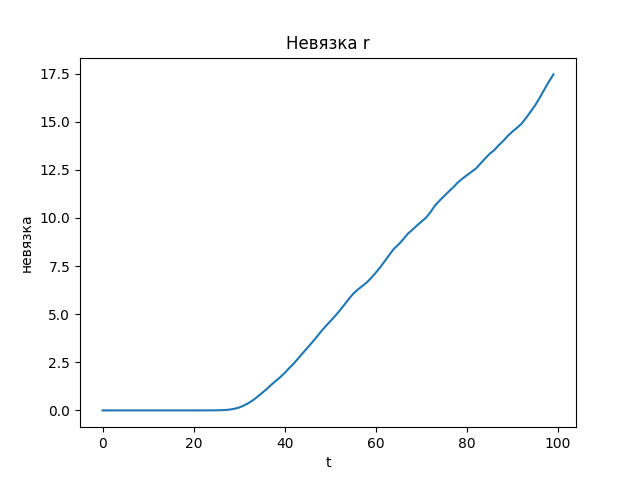
\includegraphics[width=0.8\textwidth]{rdiv.png}
\end{center}
Как видим это гораздо ближе к референсным данным( $\approx 0.21$) чем полученное прямым способом
% section из_первого_задания (end)

\section{Зависимость от термостата} % (fold)
\label{sec:зависимость_от_термостата}
Построим СКС для разных $\tau$ и поймем что происходит что-то рандомное, на бесконечности $\pm$ сходящееся к одному значению. При маленьких $t$ средняя вырывается вперед что странно, поэтому я попробовал посмотреть на больший промежуток времени 
\begin{figure}[H]
\begin{center}
\begin{minipage}[h]{0.45\linewidth}
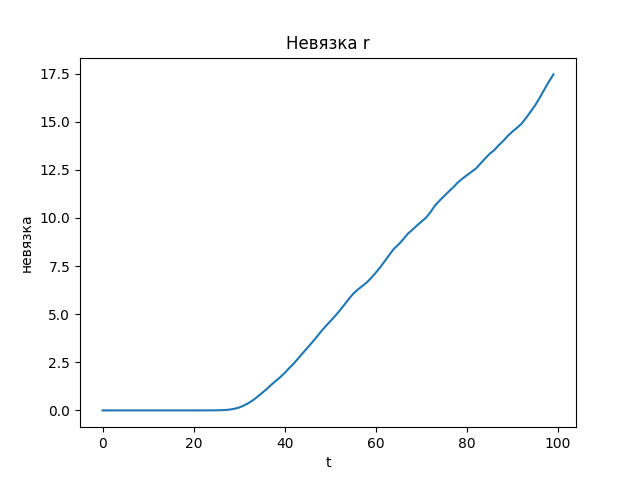
\includegraphics[width=1.1\linewidth]{rdiv.png}
\caption{СКС при $dt = 0.001$} %% подпись к рисунку
\label{ris:experimoriginal} %% метка рисунка для ссылки на него
\end{minipage}
\hfill
\begin{minipage}[h]{0.45\linewidth}
\begin{center}
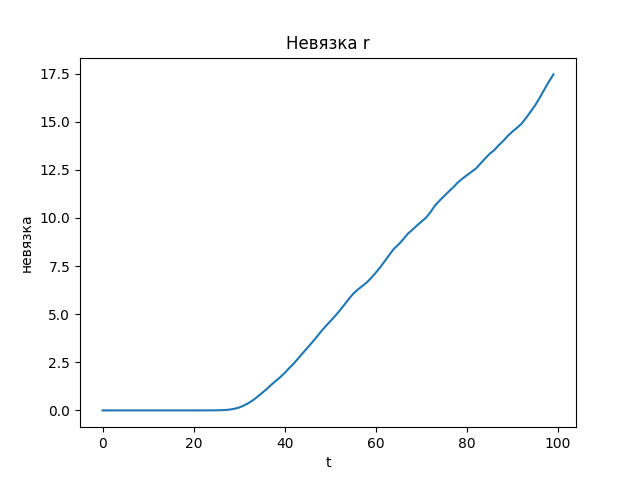
\includegraphics[width=1.1\textwidth]{rdiv.png}
\caption{СКС при $dt = 0.01$}
\end{center}
\end{minipage}
\end{center}
\end{figure}
Теперь переделаем эксперимент с LAMMPS и посмотрим на результаты
\begin{figure}[h]
\begin{center}
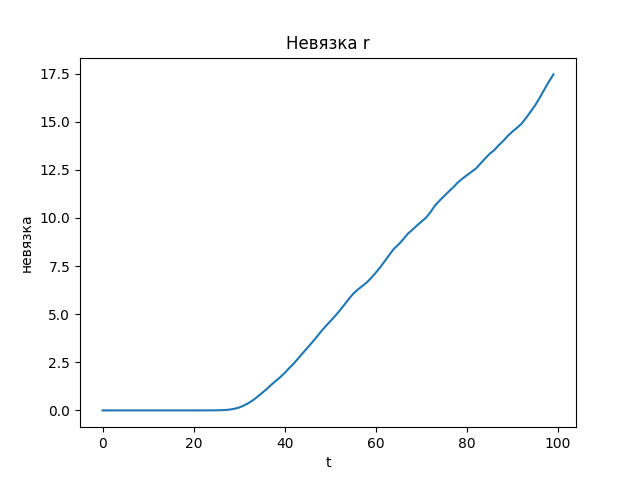
\includegraphics[width=0.7\textwidth]{rdiv.png}
\caption{СКС при $dt = 0.005$  (на пикче неправильное $dt$ )}
\end{center}
\end{figure}




\begin{figure}[H]
\begin{center}
\begin{minipage}[h]{0.65\linewidth}
Как видим СКС при $\tau = 1000$ повел себя неожиданным образом и почти сравнялся с $\tau = 100$. Однако здесь показаны СКС для отдельных симуляций, усреднение по 10 симуляциям дает адекватную зависимость. Cудя по всему следующие симуляции следует проводить с $\tau = 500$ )) Здесь брался термостат Беренсдена, вроде для него надо было $\tau$  менять
\end{minipage}
\hfill
\begin{minipage}[h]{0.25\linewidth}
 \vspace{-2ex}
\begin{table}[H]
\begin{tabular}{l|l}
$\tau$  & $D$     \\ \hline
10   & 0.135 \\ 
100  & 0.131 \\ 
500  & 0.124 \\ 
1000 & 0.123 \\ 
\end{tabular}
\end{table}
\end{minipage}
\end{center}
\end{figure}

% section зависимость_от_термостата (end)

\section{Проверка экспериментальной зависимости} % (fold)
\label{sec:проверка_экспериментальной_зависимости}
На этот раз проводилась симуляция Lammps c усреднением по 10 симуляциям, $dt = 0.005$
\begin{itemize}
    \item при $T = 0.8$ и $\rho =0.8$ $P = 0.67$ $D = 0.051$ $D_{ref} = 0.048$
    \item при $T = 0.9$ и $\rho =0.8$ $P = 1.188$ $D = 0.062$ 
    \item при $T = 0.75$ и $\rho =0.8$ $P = 0.406$ $D = 0.047$ 
\end{itemize}
Нужно проверить уравнение
\begin{equation}
    Log_{10} D = 0.05 + 0.07 P - \frac{1.04 + 0.1 P}{T}
\end{equation}


\begin{align*}
    -1.28 = -1.29\\
    -1.15 = -1.21\\
    -1.36 = -1.32
\end{align*}
Господи, оно сошлось
% section проверка_экспериментальной_зависимости (end)

\newpage
\section{Флуктуации энергии} % (fold)
\label{sec:флуктуации_энергии}
Второе получилось в прошлый раз с домашней программой, верхнее - результат из LAMMPS. Выглядит пугающе симметрично, возможно особенность дискретного преобразования Фурье, но не знаю. У меня вопрос откуда берутся члены с частотой позволяющей им несколько раз в симуляции появляться.
\begin{figure}[h]
\begin{center}
\includegraphics[width=0.9\textwidth]{ff.png}
\caption{в LAMMPS}
\end{center}
\end{figure}
\begin{figure}[h]
\begin{center}
\includegraphics[width=1\textwidth]{Figure_no.png}
\caption{моя прога без термостата}
\end{center}
\end{figure}


% section флуктуации_энергии (end)
\end{document}